\documentclass[border=10pt]{standalone}
\usepackage[svgnames]{xcolor}
\usepackage{amsmath}
\usepackage{pgfplots}
\pgfplotsset{compat=newest}
\usepackage[sfdefault]{FiraSans}
\usepackage{FiraMono}
\renewcommand*\familydefault{\sfdefault}
\begin{document}
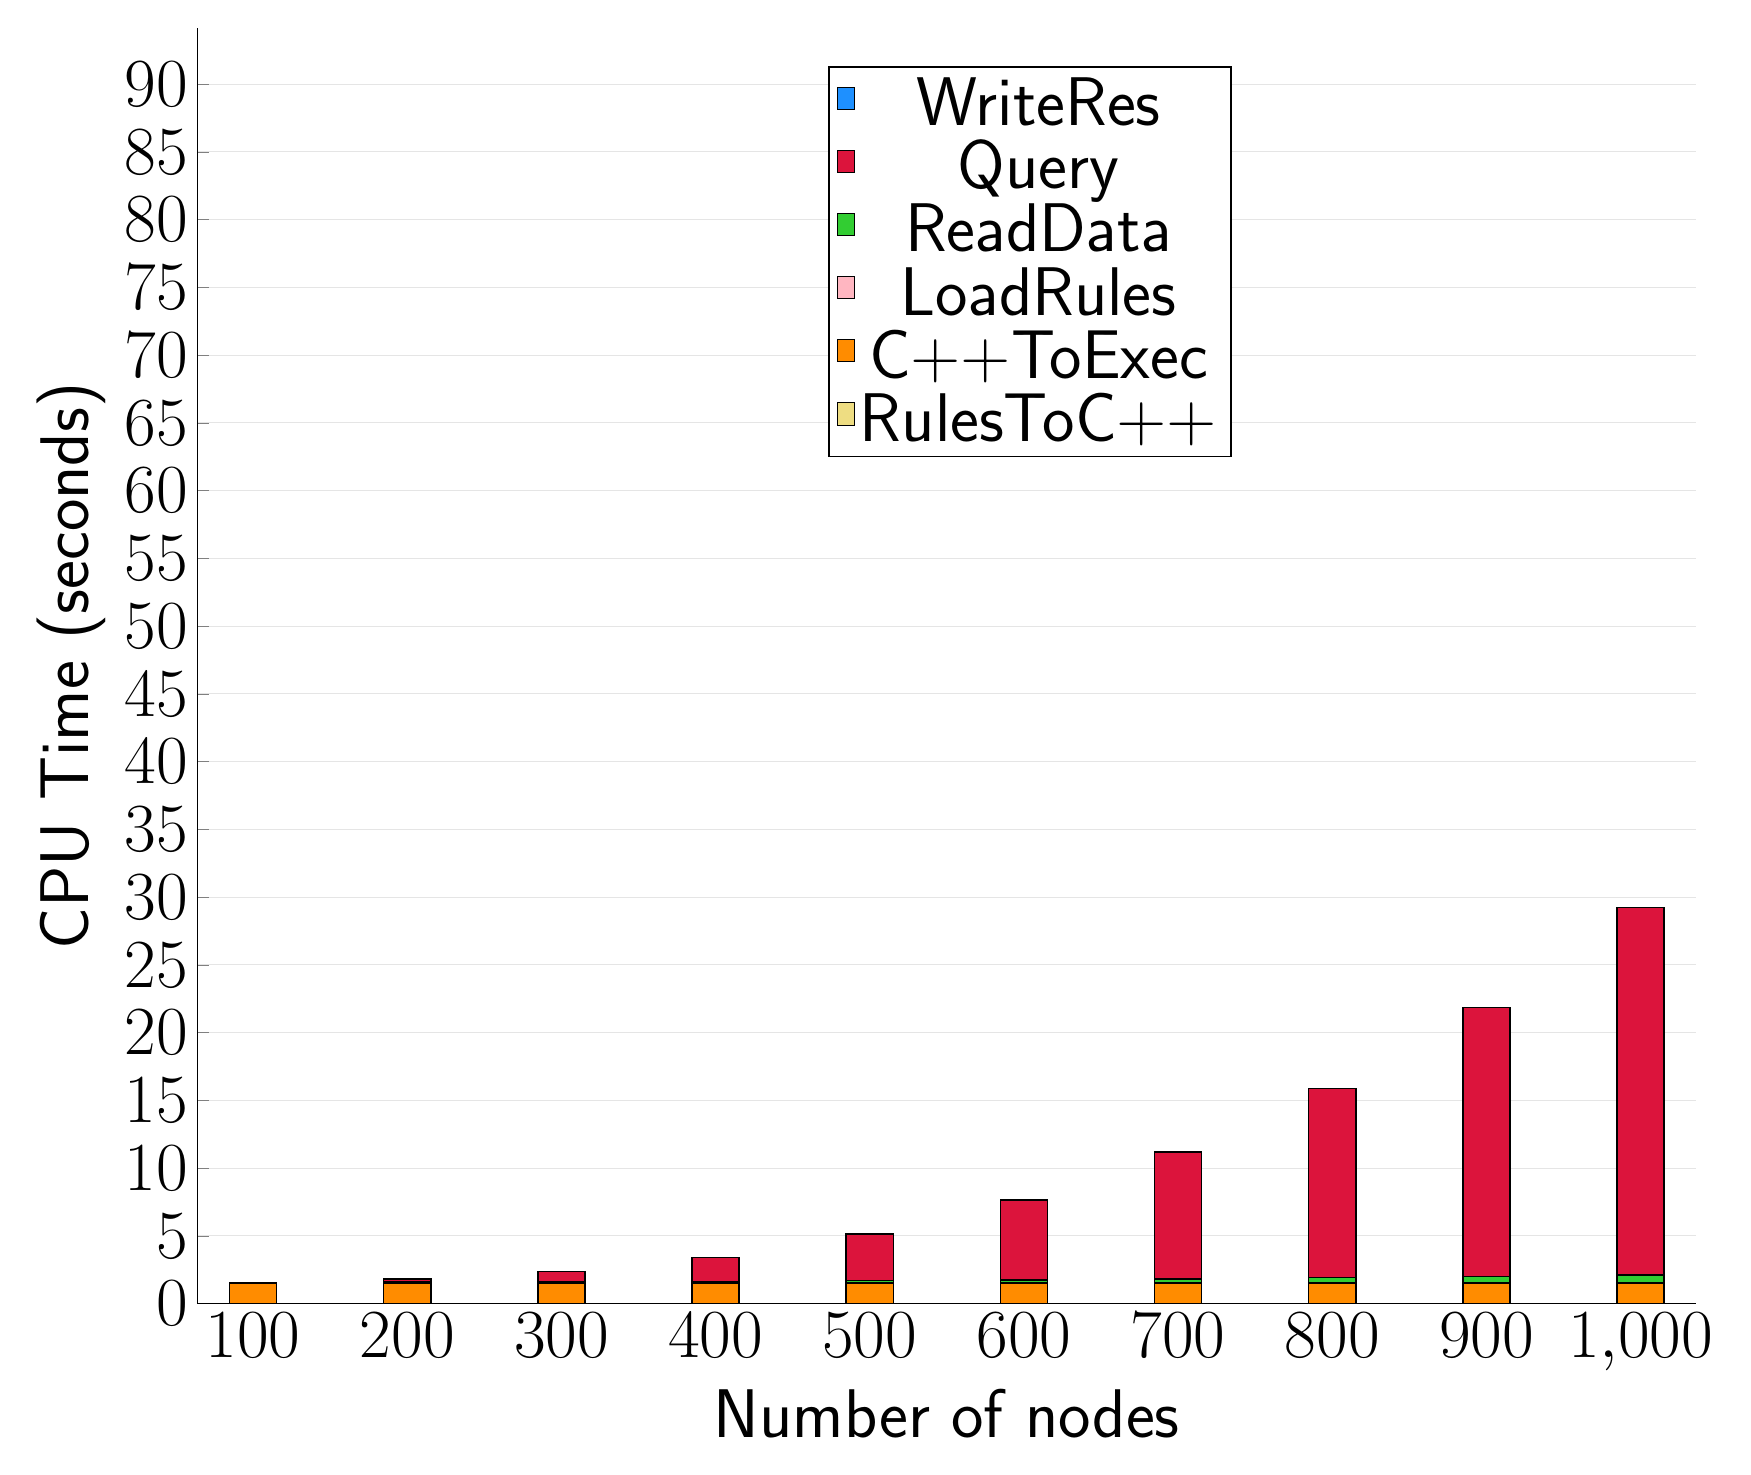
\begin{tikzpicture}
\begin{axis}[
   ybar stacked,
   width=1.7\textwidth,
   bar width=0.6cm,
   ymajorgrids, tick align=inside,
   major grid style={draw=gray!20},
   xtick=data,
   ymin=0, ymax=94.12288,
   axis x line*=bottom,
   axis y line*=left,
   enlarge x limits=0.04,
   legend style={
       at={(0.69, 0.97)},
       anchor=north east,
       legend columns=1,
       font=\Huge,
   },
   ylabel={CPU Time (seconds)},
   xlabel={Number of nodes},
   label style={font=\Huge},
   tick label style={font=\Huge},
]
\addlegendimage{fill=DodgerBlue, draw=black, line width=0.2pt}
\addlegendentry{WriteRes}
\addlegendimage{fill=Crimson, draw=black, line width=0.2pt}
\addlegendentry{Query}
\addlegendimage{fill=LimeGreen, draw=black, line width=0.2pt}
\addlegendentry{ReadData}
\addlegendimage{fill=LightPink, draw=black, line width=0.2pt}
\addlegendentry{LoadRules}
\addlegendimage{fill=DarkOrange, draw=black, line width=0.2pt}
\addlegendentry{C++ToExec}
\addlegendimage{fill=LightGoldenrod, draw=black, line width=0.2pt}
\addlegendentry{RulesToC++}
\addplot +[fill=LightGoldenrod, draw=black, line width=0.55pt] coordinates {
(100, 0.006000000000000001)
(200, 0.006000000000000001)
(300, 0.010000000000000002)
(400, 0.008000000000000002)
(500, 0.006000000000000001)
(600, 0.004000000000000001)
(700, 0.008000000000000002)
(800, 0.004000000000000001)
(900, 0.006000000000000001)
(1000, 0.004000000000000001)
};
\addplot +[fill=DarkOrange, draw=black, line width=0.55pt] coordinates {
(100, 1.5119999999999998)
(200, 1.532)
(300, 1.52)
(400, 1.5240000000000002)
(500, 1.52)
(600, 1.514)
(700, 1.52)
(800, 1.5219999999999998)
(900, 1.52)
(1000, 1.52)
};
\addplot +[fill=LightPink, draw=black, line width=0.55pt] coordinates {
(100, 0.00014160000000000003)
(200, 0.00016140000000000002)
(300, 0.00015060000000000003)
(400, 0.00013859999999999998)
(500, 0.000141)
(600, 0.00014759999999999998)
(700, 0.0001524)
(800, 0.00014)
(900, 0.0001672)
(1000, 0.00013340000000000002)
};
\addplot +[fill=LimeGreen, draw=black, line width=0.55pt] coordinates {
(100, 0.0134862)
(200, 0.040637599999999996)
(300, 0.0725744)
(400, 0.112905)
(500, 0.163064)
(600, 0.2252678)
(700, 0.300994)
(800, 0.3879516)
(900, 0.485752)
(1000, 0.595093)
};
\addplot +[fill=Crimson, draw=black, line width=0.55pt] coordinates {
(100, 0.043060799999999996)
(200, 0.2308396)
(300, 0.7538556)
(400, 1.7743120000000001)
(500, 3.4381699999999995)
(600, 5.915206)
(700, 9.360800000000001)
(800, 13.963240000000003)
(900, 19.836879999999997)
(1000, 27.09808)
};
\addplot +[fill=DodgerBlue, draw=black, line width=0.55pt] coordinates {
(100, 2.56e-05)
(200, 6.840000000000001e-05)
(300, 0.00014180000000000003)
(400, 0.0001692)
(500, 0.00017500000000000003)
(600, 0.000167)
(700, 0.00019999999999999996)
(800, 0.0001874)
(900, 0.000199)
(1000, 0.00020439999999999998)
};
\end{axis}
\end{tikzpicture}

\end{document}
